%!TEX root = ../template.tex
%%%%%%%%%%%%%%%%%%%%%%%%%%%%%%%%%%%%%%%%%%%%%%%%%%%%%%%%%%%%%%%%%%%%
%% chapter3.tex
%% NOVA thesis document file
%%
%% Chapter with a short latex tutorial and examples
%%%%%%%%%%%%%%%%%%%%%%%%%%%%%%%%%%%%%%%%%%%%%%%%%%%%%%%%%%%%%%%%%%%%

\typeout{NT FILE chapter3.tex}%

\makeatletter
\newcommand{\ntifpkgloaded}{%
  \@ifpackageloaded%
}
\makeatother


\chapter{Experiment}
\label{cha:experiment}

\epigraph{
	"Somewhere, something incredible is waiting to be known."
}{Carl Sagan}



\section{Context and Goal of the Experiment} % (fold)
\label{sec:contex_goal_experiment}

The proposed experiment, detailed in research proposal G-24-00249 \cite{panin2024neutron}, aims to investigate the structure of the neutron-rich fluorine isotope, $^{25}$F, through one-proton knockout reactions. This study is motivated by the "drastic extension of the neutron drip line for Z=9 compared to Z=8 isotopes," a phenomenon that remains poorly understood \cite{ahn_location_2019}. The experiment seeks to elucidate how the $^{24}$O core is polarized by the presence of an additional proton in $^{25}$F, thereby shedding light on the mechanisms responsible for the observed drip line extension.

The experiment will employ the quasi-free scattering (\gls{QFS}) reaction $^{25}$F(p,2p)$^{24}$O in inverse kinematics, effectively knocking out a deeply bound valence proton from the $^{25}$F nucleus \cite{panin_exclusive_2016}. This approach will utilize the \gls{R3B} experimental setup, including the high-efficiency neutron detector NeuLAND \cite{boretzky_neuland_2021}, to achieve complete kinematic measurements and obtain accurate spectroscopic information on the populated final states of $^{24}$O. By analyzing the experimental data, researchers aim to determine the extent to which the single $d_{5/2}$ proton in $^{25}$F modifies the structure of the core nucleons, potentially indicating deformation or polarization of the $^{24}$O core \cite{macchiavelli_core_2020}.

Ultimately, the goal of this experiment is to provide a more detailed understanding of the nuclear structure of neutron-rich fluorine isotopes and the underlying reasons for the extended neutron drip line at Z=9. The results will contribute to a more comprehensive picture of nuclear forces and structure in exotic nuclei, addressing a fundamental question in nuclear physics.


\begin{figure}
	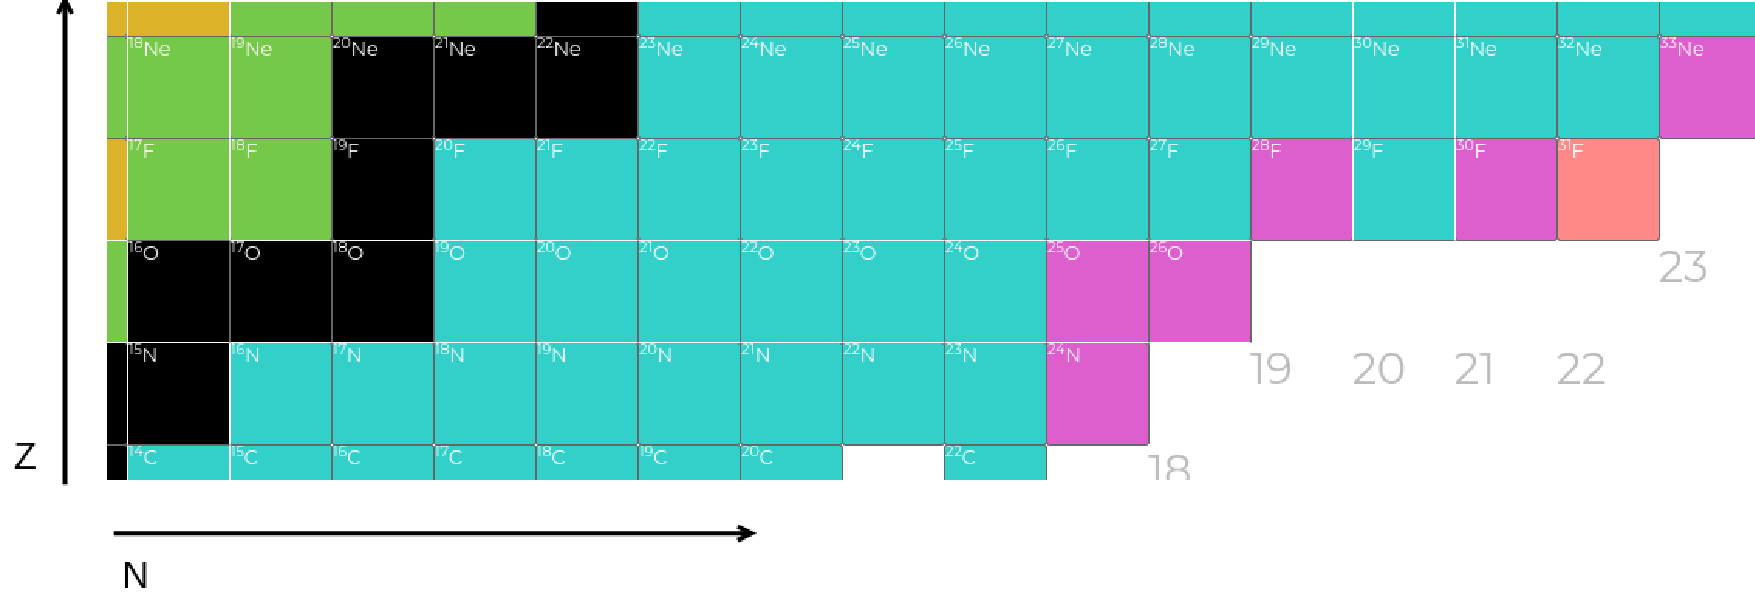
\includegraphics[width=\linewidth]{NeutronDripLine}
	\caption{Visualization of the neutron drip line extension from oxygen to fluorine. The extended neutron-rich limit for fluorine isotopes illustrates how additional protons influence nuclear binding near the drip line. Figure adapted from the IAEA Live Chart of Nuclides \cite{IAEA_NuclideChart}.}
	\label{fig:NeutronDripLine}
\end{figure}


\section{The GSI Accelerator System}
%Annex \ref{ann:gsi_facility}

The previously described experiment will take place at the GSI Helmholtzzentrum für Schwerionenforschung in Darmstadt, Germany. GSI’s accelerator complex, seen in Figure \ref{fig:GSI}, provides the infrastructure required to produce and deliver rare isotope beams, such as $^{25}$F, for inverse kinematics reactions. The \gls{R3B} setup, located in Cave C downstream of the FRS, enables complete kinematic reconstruction, making it well-suited for the spectroscopic investigation of exotic nuclei. The following sections outline the accelerator chain that delivers these beams—from ion production through the UNILAC and SIS18 to the FRS and the experimental area.

\begin{figure}
	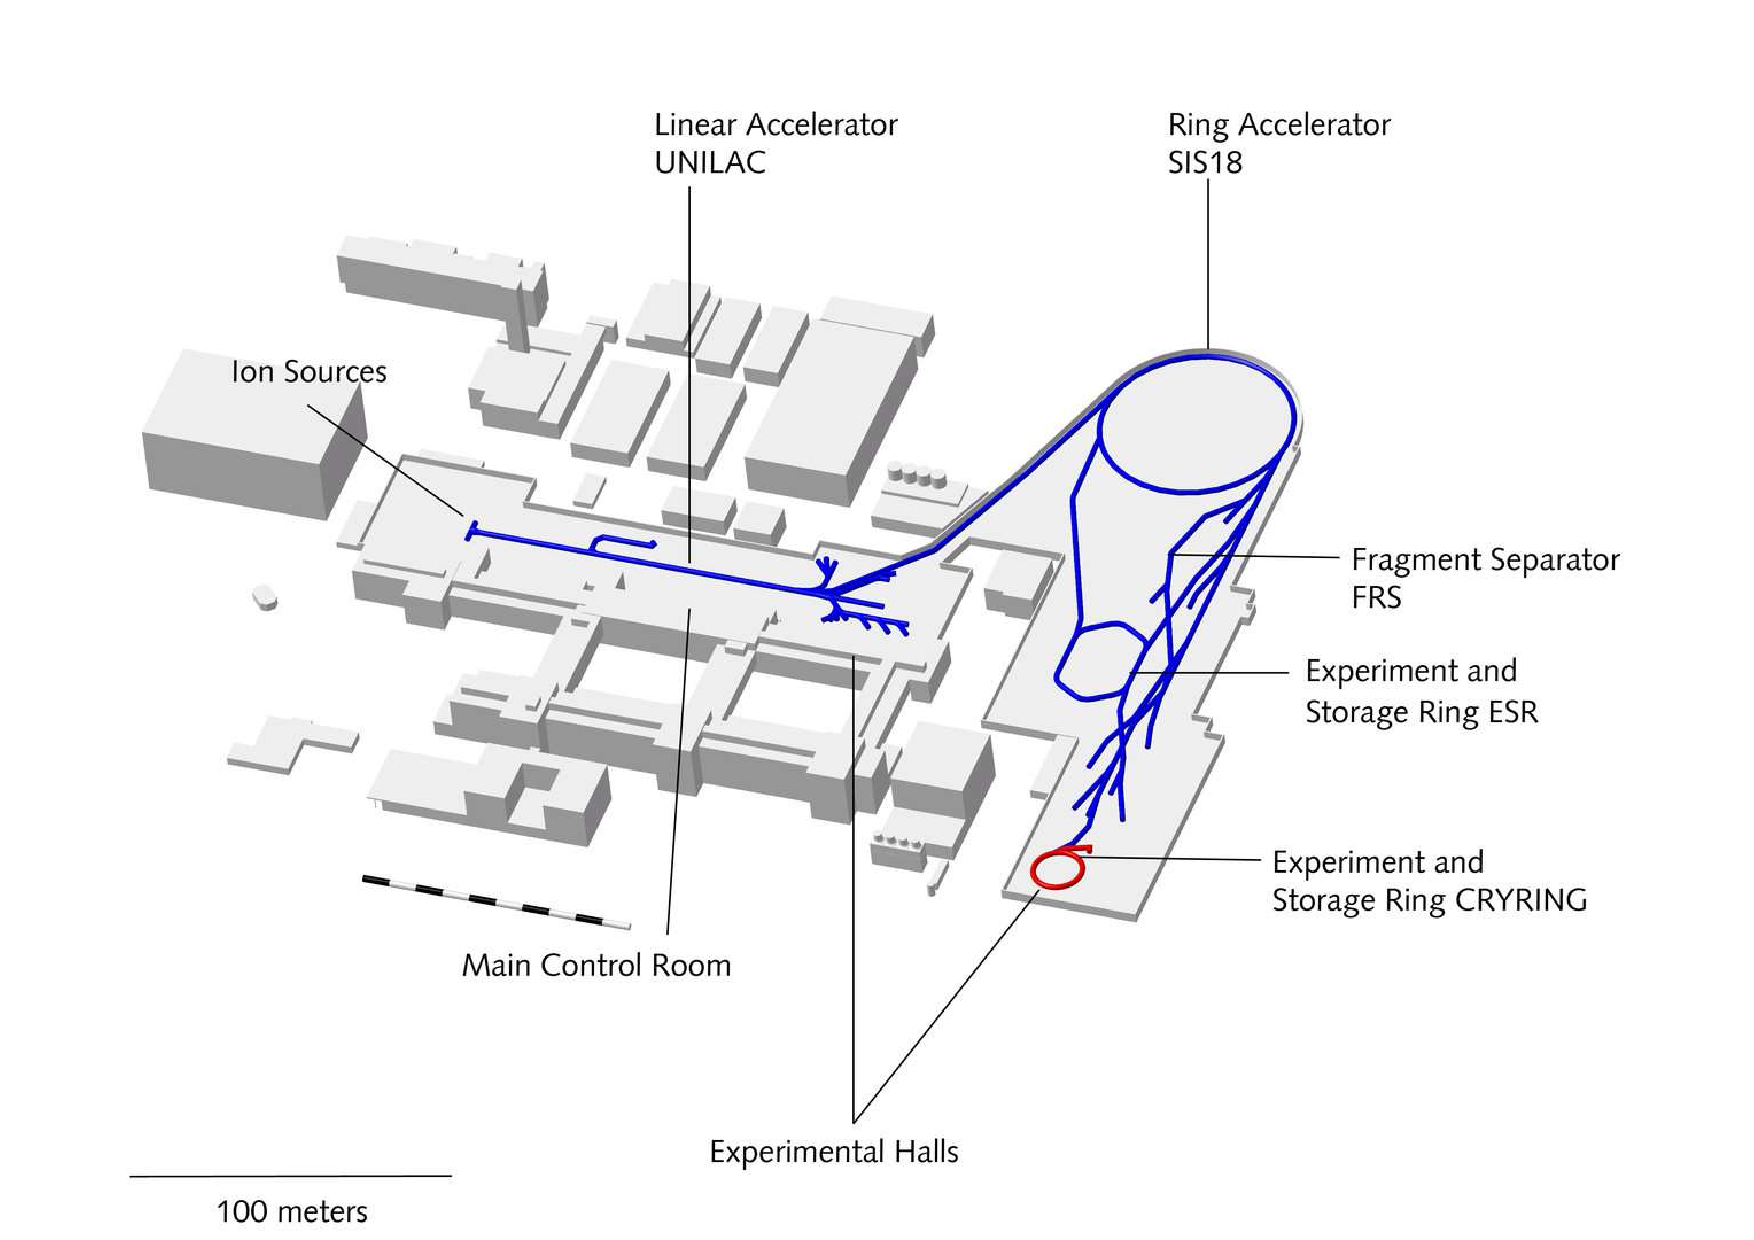
\includegraphics[width=\linewidth]{GSI}
	\caption{Schematic layout of the GSI Helmholtzzentrum accelerator facility. The diagram shows the major components including the ion sources, the UNILAC linear accelerator, the SIS18 synchrotron, the Fragment Separator (FRS), and the associated experimental halls \cite{gsiAcceleratorFacility}.}
	\label{fig:GSI}
\end{figure}


\subsection{From Source to Experimental Cave}

\subsubsection{Ion Production}

The accelerator cycle begins with the production of ions in specialized ion sources. Depending on the experimental requirements, different types of sources are used, including electron cyclotron resonance (ECR) sources and Penning ion sources \cite{hollinger_status_2008}. These generate high charge state ions by stripping electrons from atoms in a plasma environment. The produced ions are pre-accelerated and then injected into the linear accelerator for further acceleration.


\subsubsection{The UNILAC}

The Universal Linear Accelerator (UNILAC) \cite{vormann_high_2023} serves as the primary injector for the GSI accelerator chain. It accelerates ions to energies of several MeV/u before their injection into the synchrotron. Structurally, the UNILAC consists of several stages: a radio-frequency quadrupole (RFQ), an interdigital H-mode drift tube linac (IH-DTL), and a transfer line to the synchrotron SIS18 \cite{barth_high_2022}. Over the years, substantial upgrades have been implemented to accommodate high-intensity beams and improve the beam quality for heavy ion acceleration . The layout of the UNILAC and its role as the front-end of the accelerator chain is depicted in Figure \ref{fig:UNILAC}.


\begin{figure}
	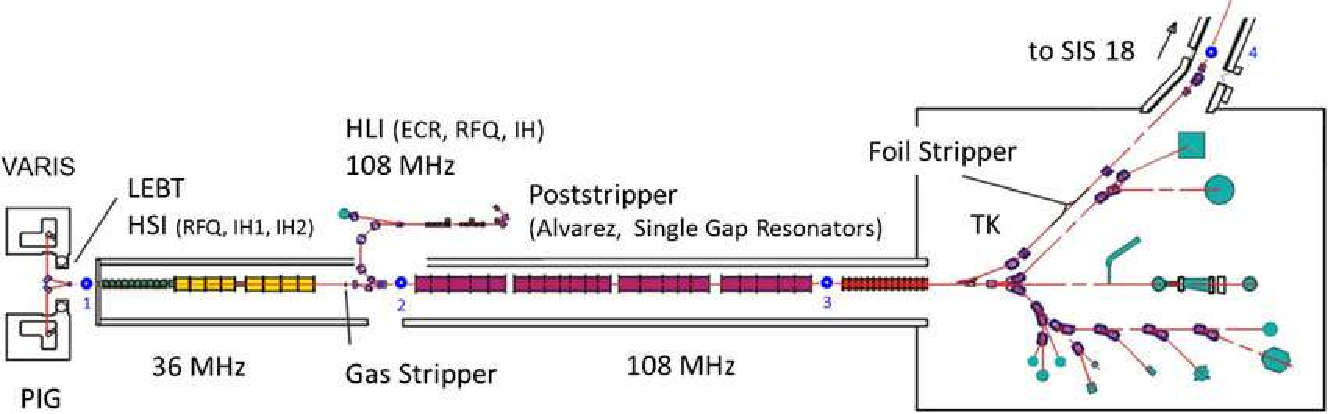
\includegraphics[width=\linewidth]{UNILAC}
	\caption{Detailed schematic of the UNILAC accelerator. The figure highlights the beamline structure from ion sources through the High Current Injector (HSI), Radio-Frequency Quadrupole (RFQ), Interdigital H-mode Drift Tube Linacs (IH-DTL), gas stripper section, Alvarez Drift Tube Linac (DTL), and the transfer line to SIS18. Beam diagnostic and stripping sections are also labeled \cite{barth_high_2022}.}
	\label{fig:UNILAC}
\end{figure}


\subsubsection{The SIS18}

Following pre-acceleration by the UNILAC, ion beams are injected into the SIS18 synchrotron \cite{singh2014tune}, where they are further accelerated to relativistic energies. The SIS18 is a fast-cycling synchrotron with a magnetic rigidity of up to 18 Tm, capable of accelerating ions to several hundred MeV/u. It incorporates sophisticated beam manipulation techniques including bunch compression and multiturn injection to optimize performance and beam delivery. Figure \ref{fig:SIS18} illustrates the SIS18 layout and its specifications. The synchrotron serves both as a terminal accelerator for in-house experiments and as an injector for future FAIR components.

\begin{figure}
	\centering
	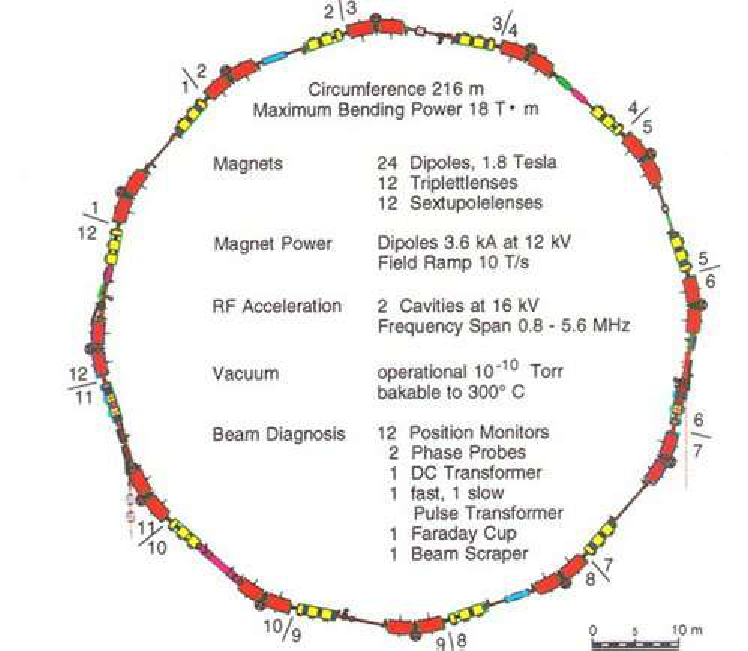
\includegraphics[width=0.7\linewidth]{SIS18}
	\caption{Plan view of the SIS18 heavy-ion synchrotron, illustrating its 12 identical lattice sections, dipole and quadrupole magnet configurations, RF acceleration cavities, and positions of beam diagnostic systems \cite{gsiSIS18Sections}.}
	\label{fig:SIS18}
\end{figure}

\subsubsection{The Fragment Separator (FRS)}

High-energy ions exiting the SIS18 are directed to the \gls{FRS} \cite{geissel_experiments_2008}, a magnetic spectrometer designed for in-flight separation of rare isotopes. The FRS exploits differences in magnetic rigidity and energy loss to isolate specific nuclear species from a cocktail beam. It comprises four dipole magnets forming a two-stage separation system and includes focal planes for tracking, time-of-flight, and energy-loss measurements . As shown in Figure \ref{fig:FRS}, the FRS facilitates beam transport from SIS18 to various experimental areas, enabling studies of exotic nuclei and reaction mechanisms.


\begin{figure}
	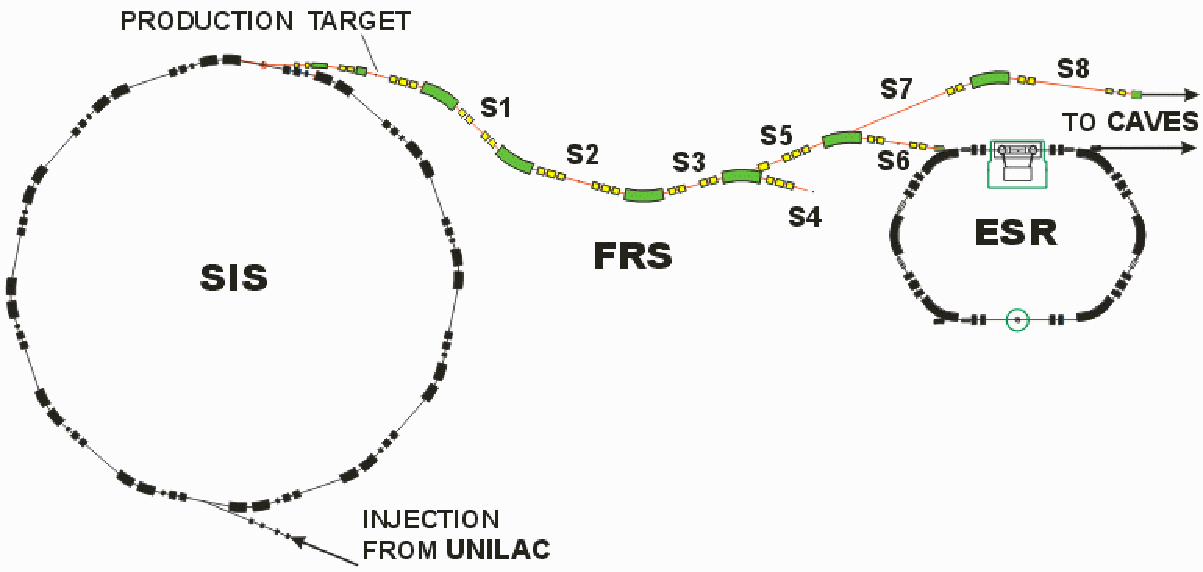
\includegraphics[width=\linewidth]{FRS}
	\caption{Schematic of the FRS system showing its dipole magnet sections, dispersive and achromatic focal planes (F1–F8), and the separation of rare isotope beams. The figure also shows the branching to dedicated experimental areas, including the Direct Branch, Ring Branch (ESR), and the experimental caves \cite{gsiWebHomelt}.}
	\label{fig:FRS}
\end{figure}


\subsubsection{Experimental Caves}

Following separation in the \gls{FRS}, ion beams are directed toward a suite of experimental stations, commonly referred to as experimental caves. These caves are equipped for diverse research programs ranging from nuclear structure and astrophysics to plasma physics and medical applications. One of the principal experimental areas is Cave C, located directly downstream of the FRS. This cave is the one that hosts the \gls{R3B} setup.

Cave C serves as a prototype environment for the future NUSTAR experiments at \gls{FAIR}. Specifically, the \gls{R3B} instrumentation and experimental approach implemented at GSI are being used to develop and validate detector technologies and methodologies for the NUSTAR Cave under construction at \gls{FAIR}. This strategic continuity ensures a seamless transition of experimental capabilities and scientific objectives from the current GSI facility to the \gls{FAIR} complex.

The overall layout of the GSI accelerator chain and its future integration with FAIR, including the locations of Cave C and the planned NUSTAR cave, is illustrated in Figure \ref{fig:GSI_FAIR_R3B}.

\begin{figure}
	\centering
	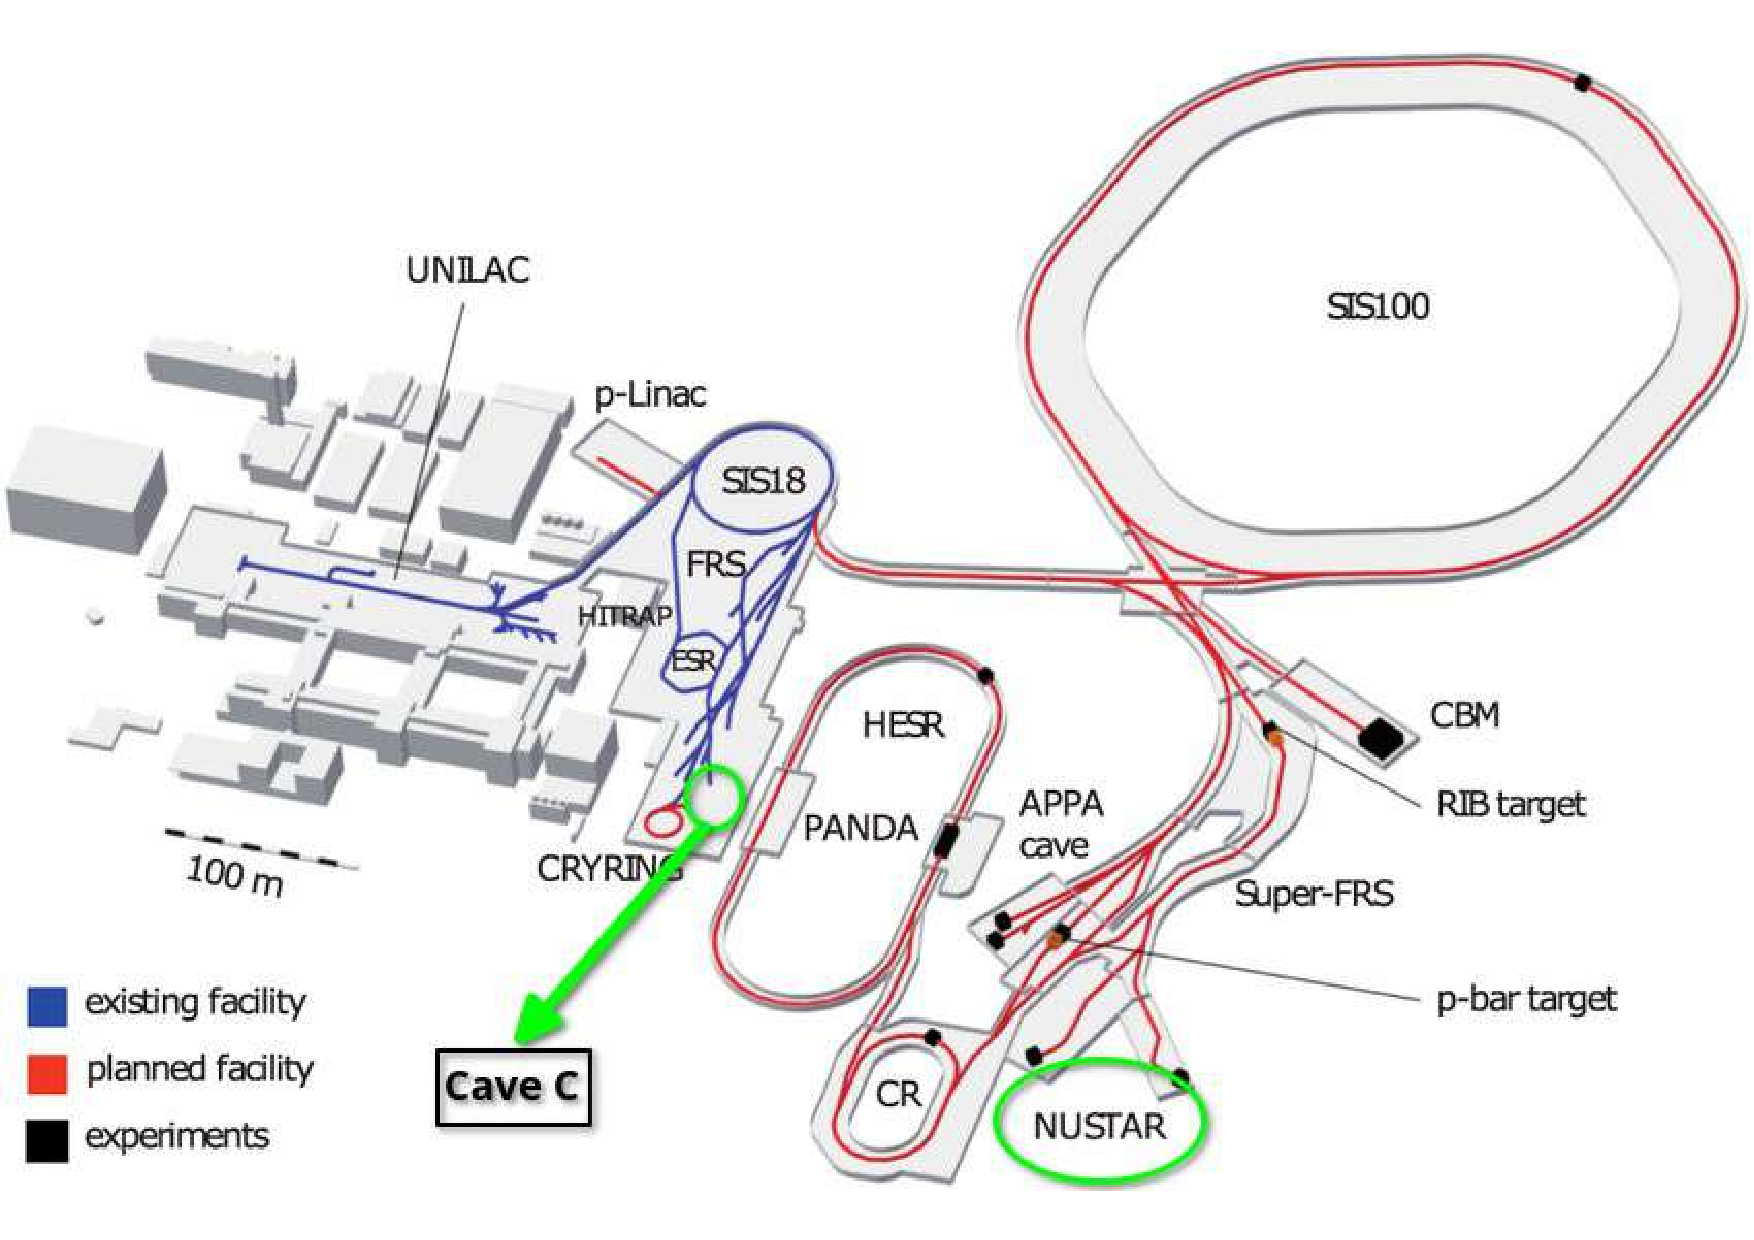
\includegraphics[width=0.8\linewidth]{FAIR_R3B}
	\caption{Layout of GSI-FAIR with Cave C highlighted, where the prototype of the future NUSTAR R$^3$B setup stands and where the present experiment took place.}
	\label{fig:GSI_FAIR_R3B}
\end{figure}


\subsubsection{Summary}

The GSI accelerator system exemplifies a complex yet highly coordinated infrastructure, progressing from ion production through successive acceleration stages and culminating in precision experiments. The integration of the UNILAC, SIS18, and \gls{FRS} ensures the delivery of high-intensity, high-quality ion beams, establishing GSI as a cornerstone of heavy ion research.



\subsection{Beam used in Experiment}

In the proposed experiment \cite{panin2024neutron}, a $^{40}$Ar primary beam with an energy of 700 MeV/u is employed to produce a secondary beam containing the $^{25}$F isotope of interest. The primary beam impinges on a beryllium target located at the \gls{FRS}, inducing nuclear fragmentation reactions. This process generates a cocktail beam consisting of various isotopes, including $^{25}$F, which is then selected and guided towards the experimental setup in Cave C.

The \gls{FRS} is used to separate and purify the secondary beam, ensuring a sufficient intensity of $^{25}$F for the subsequent experiment. As seen in Figure \ref{fig:CocktailBeam}, LISE++ simulations, using the EPAX3.1a production model, predict an intensity of approximately 30 ions per second (pps) of $^{25}$F on the secondary target \cite{panin2024neutron}. The total intensity of the secondary cocktail beam in Cave C is expected to be below 700 pps, with a purity of around 5\% for $^{25}$F \cite{panin2024neutron}. The relatively low total intensity allows for data acquisition without significant downscaling of triggers and minimizes dead time.

In Cave C, the $^{25}$F secondary beam interacts with a liquid hydrogen (LH2) target, which serves as the reaction target for the one-proton knockout reaction $^{25}$F(p,2p)$^{24}$O. The LH2 target is positioned in the center of the CALIFA calorimeter, enabling the detection of outgoing protons from the reaction. The use of a 150 mm thick LH2 cell was initially planned but, due to problems in the liquefaction phase, the cell was replaced for a 50 mm one, reducing the reaction yield. 

%The use of a 150 mm thick LH2 cell maximizes the reaction yield, compensating for the low intensity of the $^{25}$F beam.

\begin{figure}
	\centering
	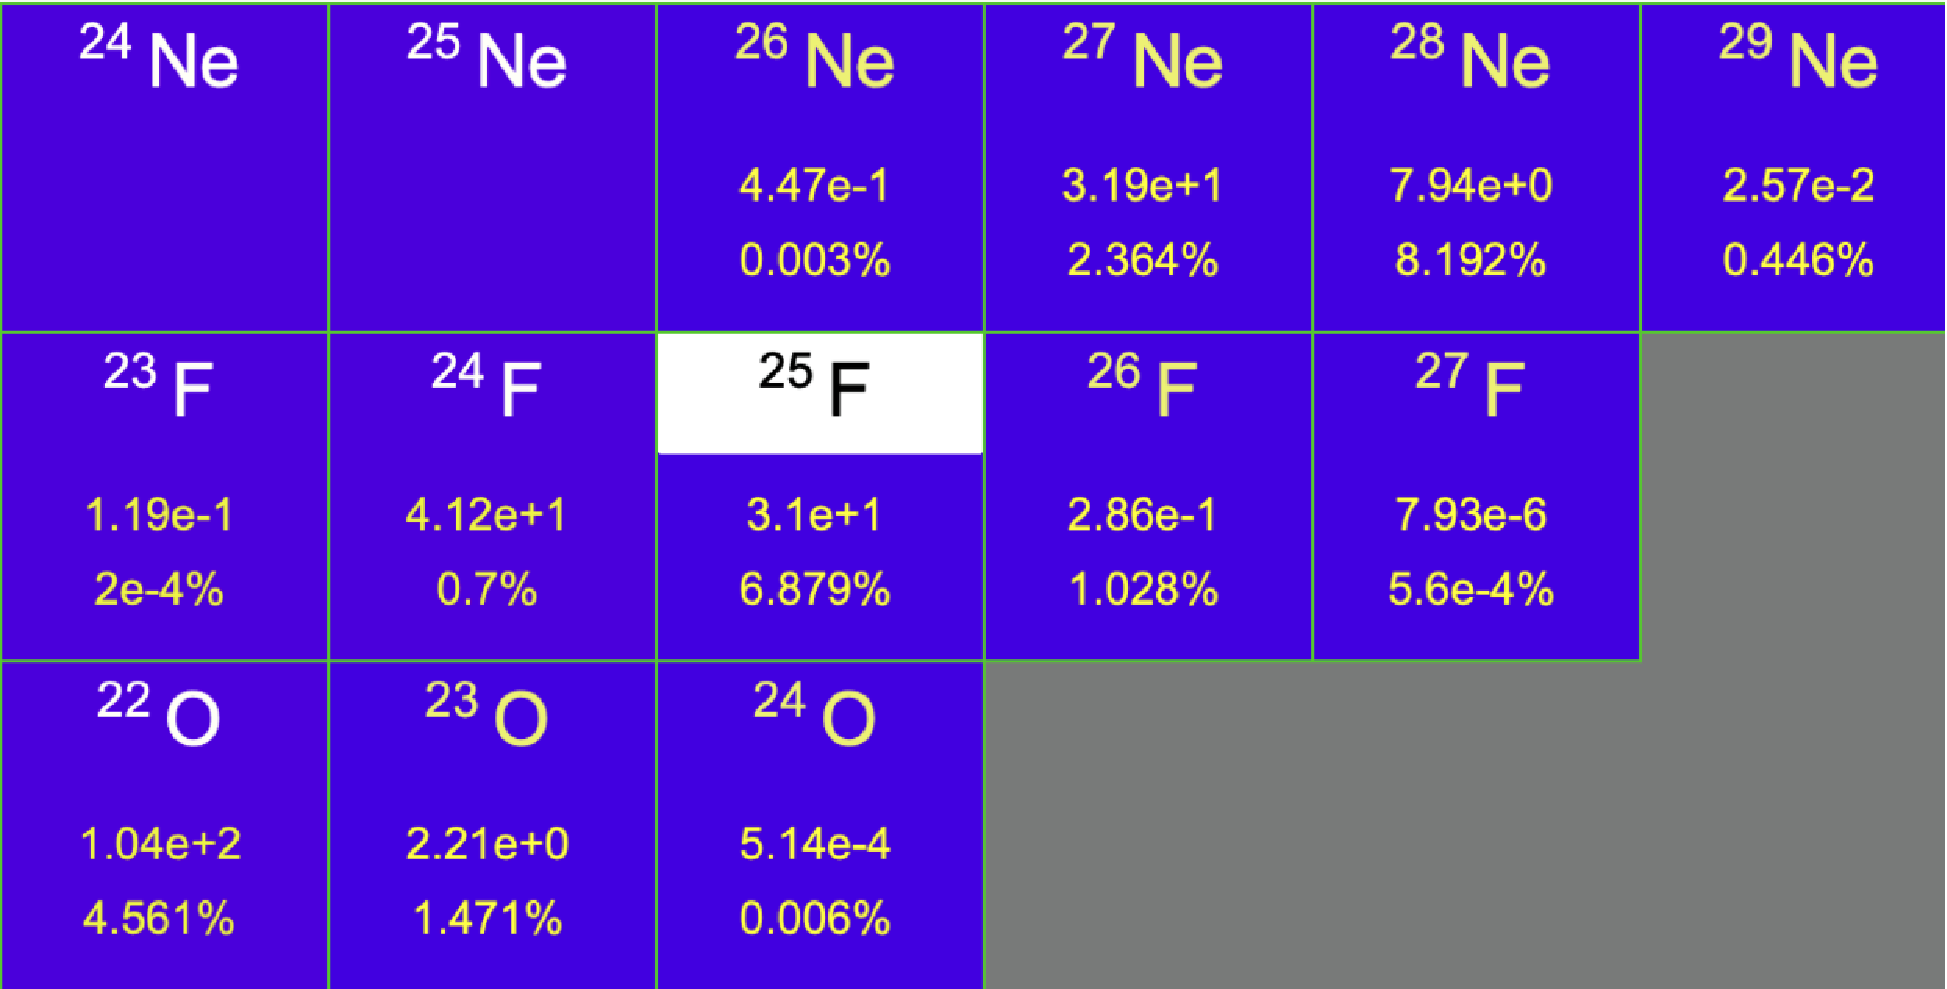
\includegraphics[width=0.75\linewidth]{CocktailBeam}
	\caption{Expected secondary cocktail beam of $^{25}$F in Cave C as obtained by LISE++ calculations. The numbers under the names of isotopes indicate calculated rates per second. Reprinted figure from Ref. \cite{panin2024neutron}.}
	\label{fig:CocktailBeam}
\end{figure}


\section{R$^3$B Setup}

%The \gls{R3B} (Reactions with Relativistic Radioactive Beams) experimental setup at GSI is designed for kinematically complete measurements of nuclear reactions involving fast exotic beams. It integrates a series of tracking and particle-identification detectors, calorimeters, spectrometers, and neutron detectors. In the present experiment, the detectors are arranged along the beamline to capture the full final-state topology of the quasi-free scattering reaction $^{25}$F(p,2p)$^{24}$O, allowing precise reconstruction of reaction kinematics and spectroscopy of the residual nucleus.

The \gls{R3B} (Reactions with Relativistic Radioactive Beams) setup at GSI is designed for high-precision, kinematically complete measurements of nuclear reactions involving rare isotope beams at relativistic energies. For the investigation of the $^{25}$F(p,2p)$^{24}$O reaction, the configuration is optimized to detect all relevant particles emerging from the target—charged fragments, recoil protons, and neutrons—with high resolution and full angular coverage. The following description reflects the actual experimental layout, based on the schematic shown in Figure \ref{fig:ExperimentalSetupSketch}, and supported by the experimental proposal and detector-specific references.

%\begin{figure}
%	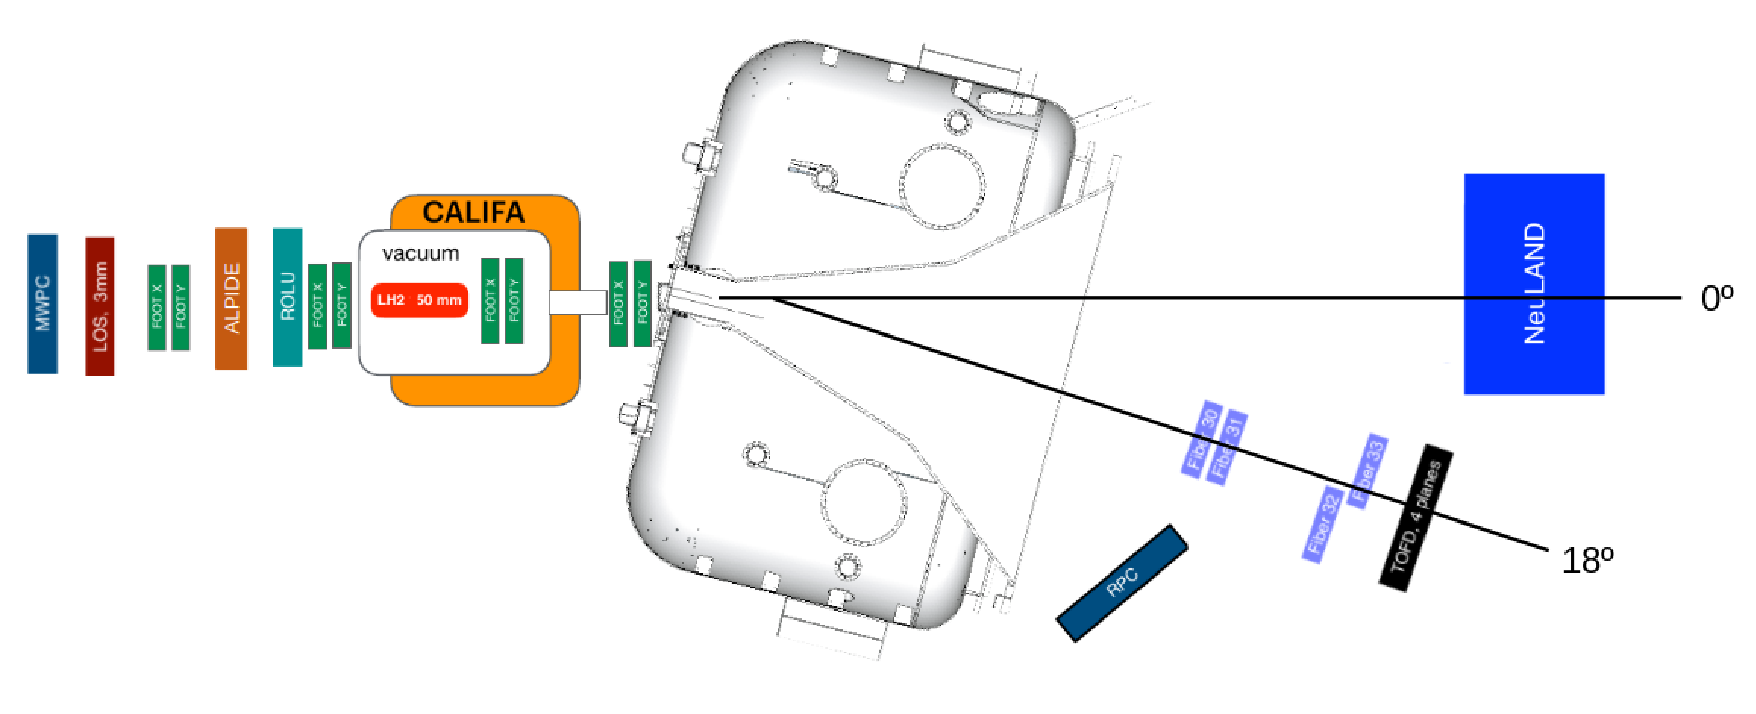
\includegraphics[width=\linewidth]{ExperimentalSetupSketch}
%	\caption{Sketch of the experimental setup at R$^3$B.} %Reprinted figure from Ref. \cite{panin2024neutron}.}
%	\label{fig:ExperimentalSetupSketch}
%\end{figure}

%\begin{figure}
%	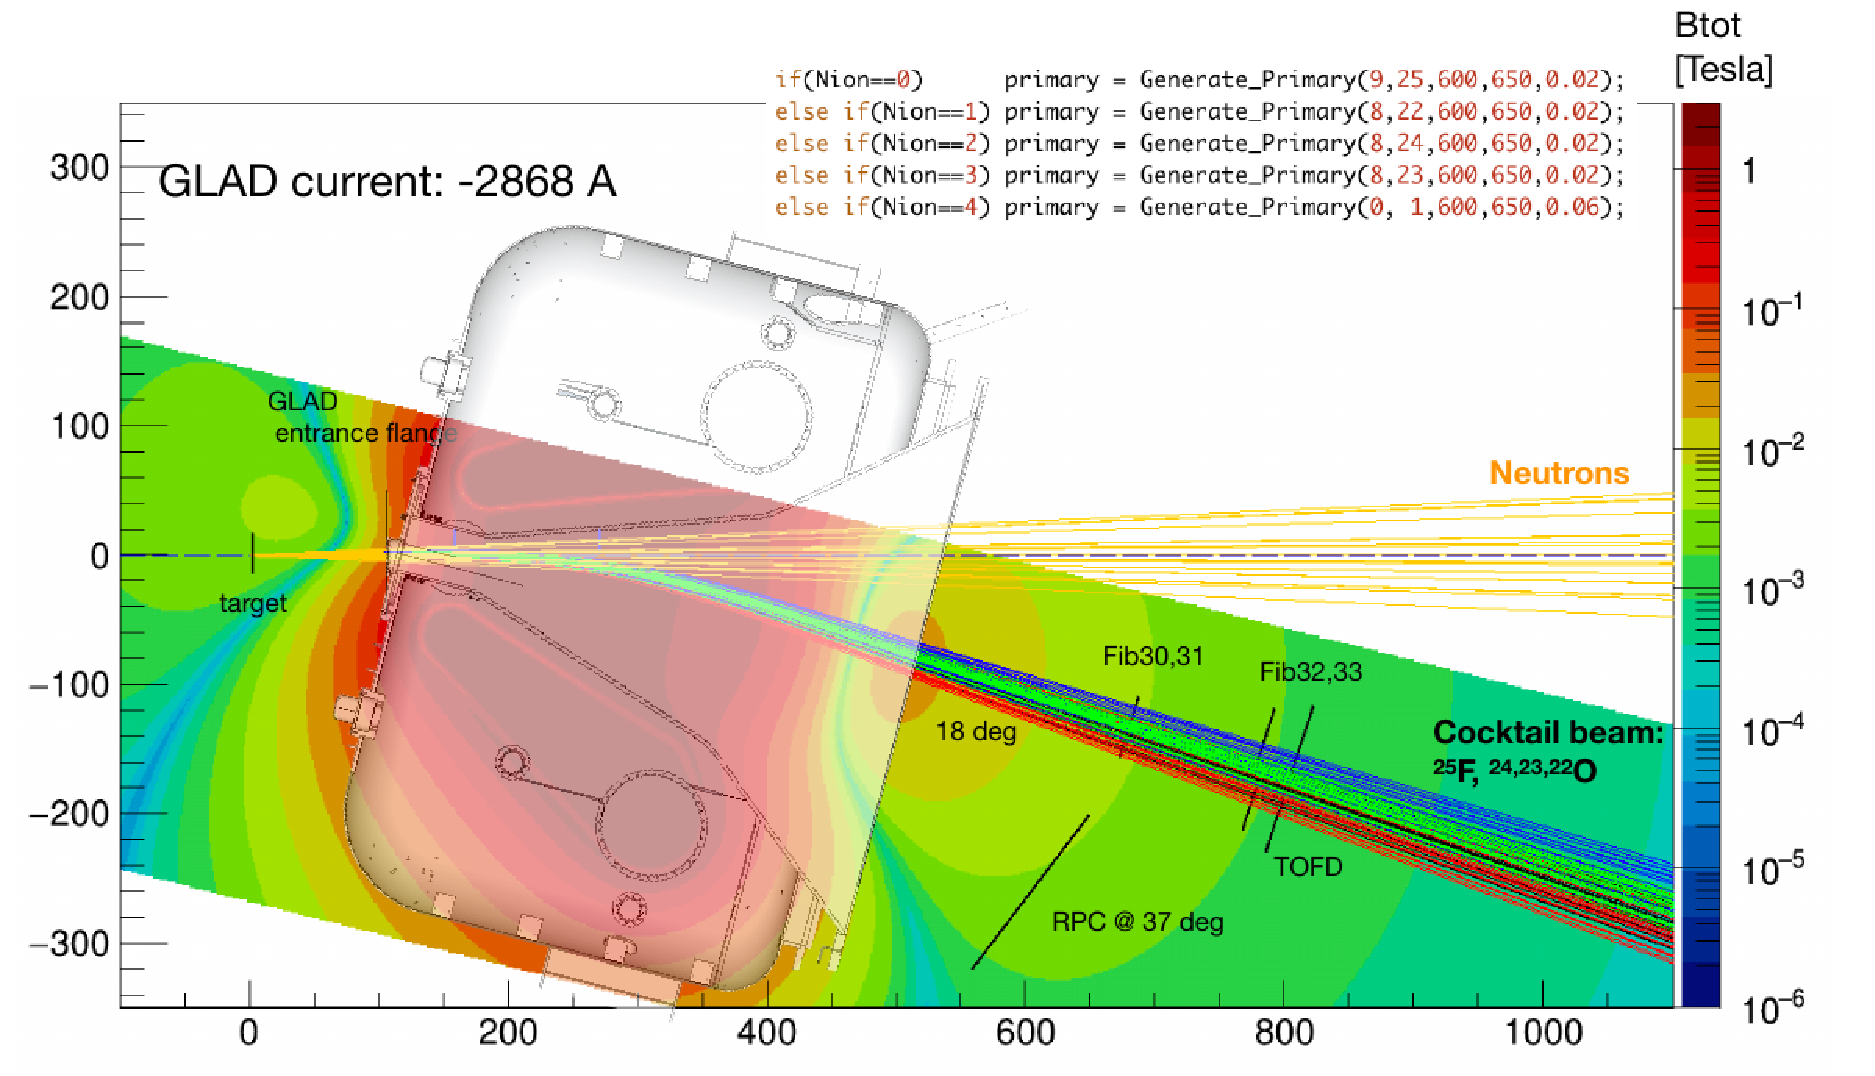
\includegraphics[width=\linewidth]{TrajectorySimulations}
%	\caption{Simulated trajectories through the GLAD magnet. The color map indicates the magnetic
%		field of the magnet. The LH2 target is located at the (0,0,0) point in front of GLAD. Reprinted figure from Ref. \cite{panin2024neutron}.}
%	\label{fig:TrajectorySimulations}
%\end{figure}



%\begin{newpdflayout}{210mm}{297mm}%{420mm}
	
%	\begin{figure}
%		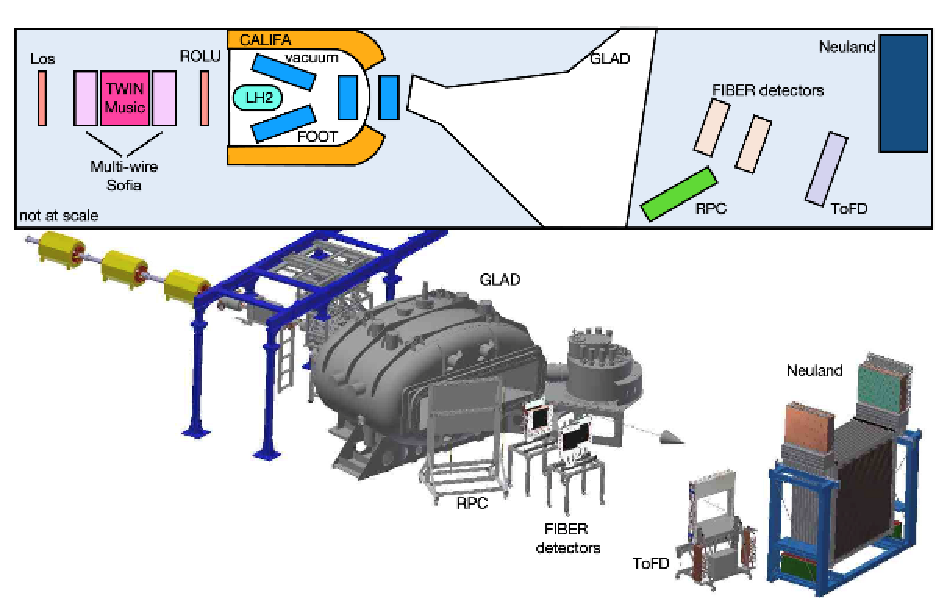
\includegraphics[width=\linewidth]{R3BSetup}
%		\caption{}
%		\label{fig:R3B_Setup}
%	\end{figure}

%\end{newpdflayout}

\begin{newpdflayout}{210mm}{297mm}%{420mm}
	
	\begin{figure}
		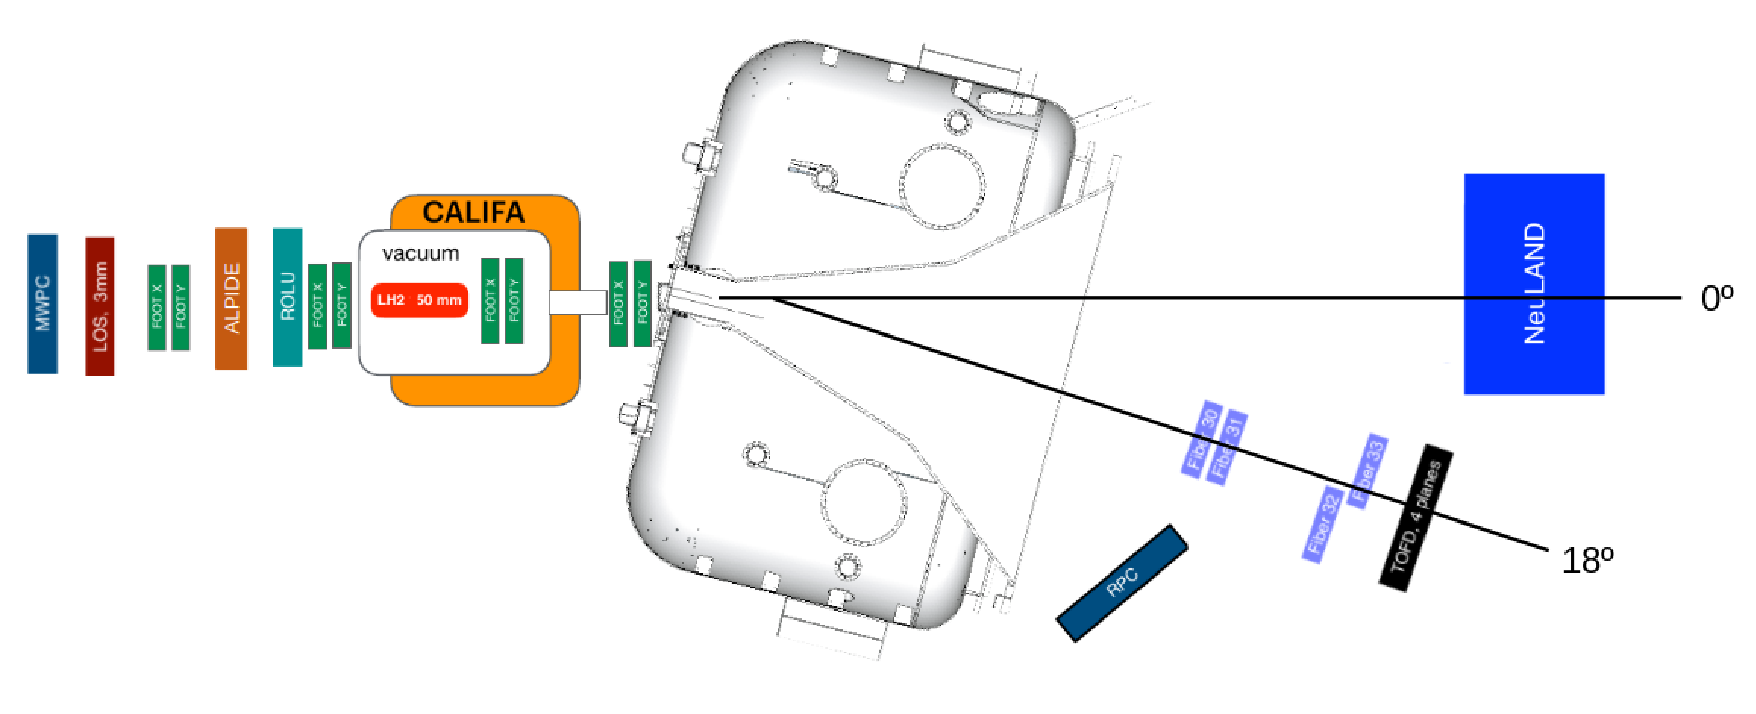
\includegraphics[width=\linewidth]{ExperimentalSetupSketch}
		\caption{Sketch of the experimental setup at R$^3$B.}
		\label{fig:ExperimentalSetupSketch}
	\end{figure}
	
\end{newpdflayout}

%\gls{R3B}

%\gls{R3B}

%\gls{ToFD}

%\gls{ToFD}

%\gls{NeuLAND}

%\gls{NeuLAND}

%\gls{GLAD}

%\gls{GLAD}

%\gls{CALIFA}

%\gls{CALIFA}

%\gls{RPC}

%\gls{RPC}
%\begin{figure}
%	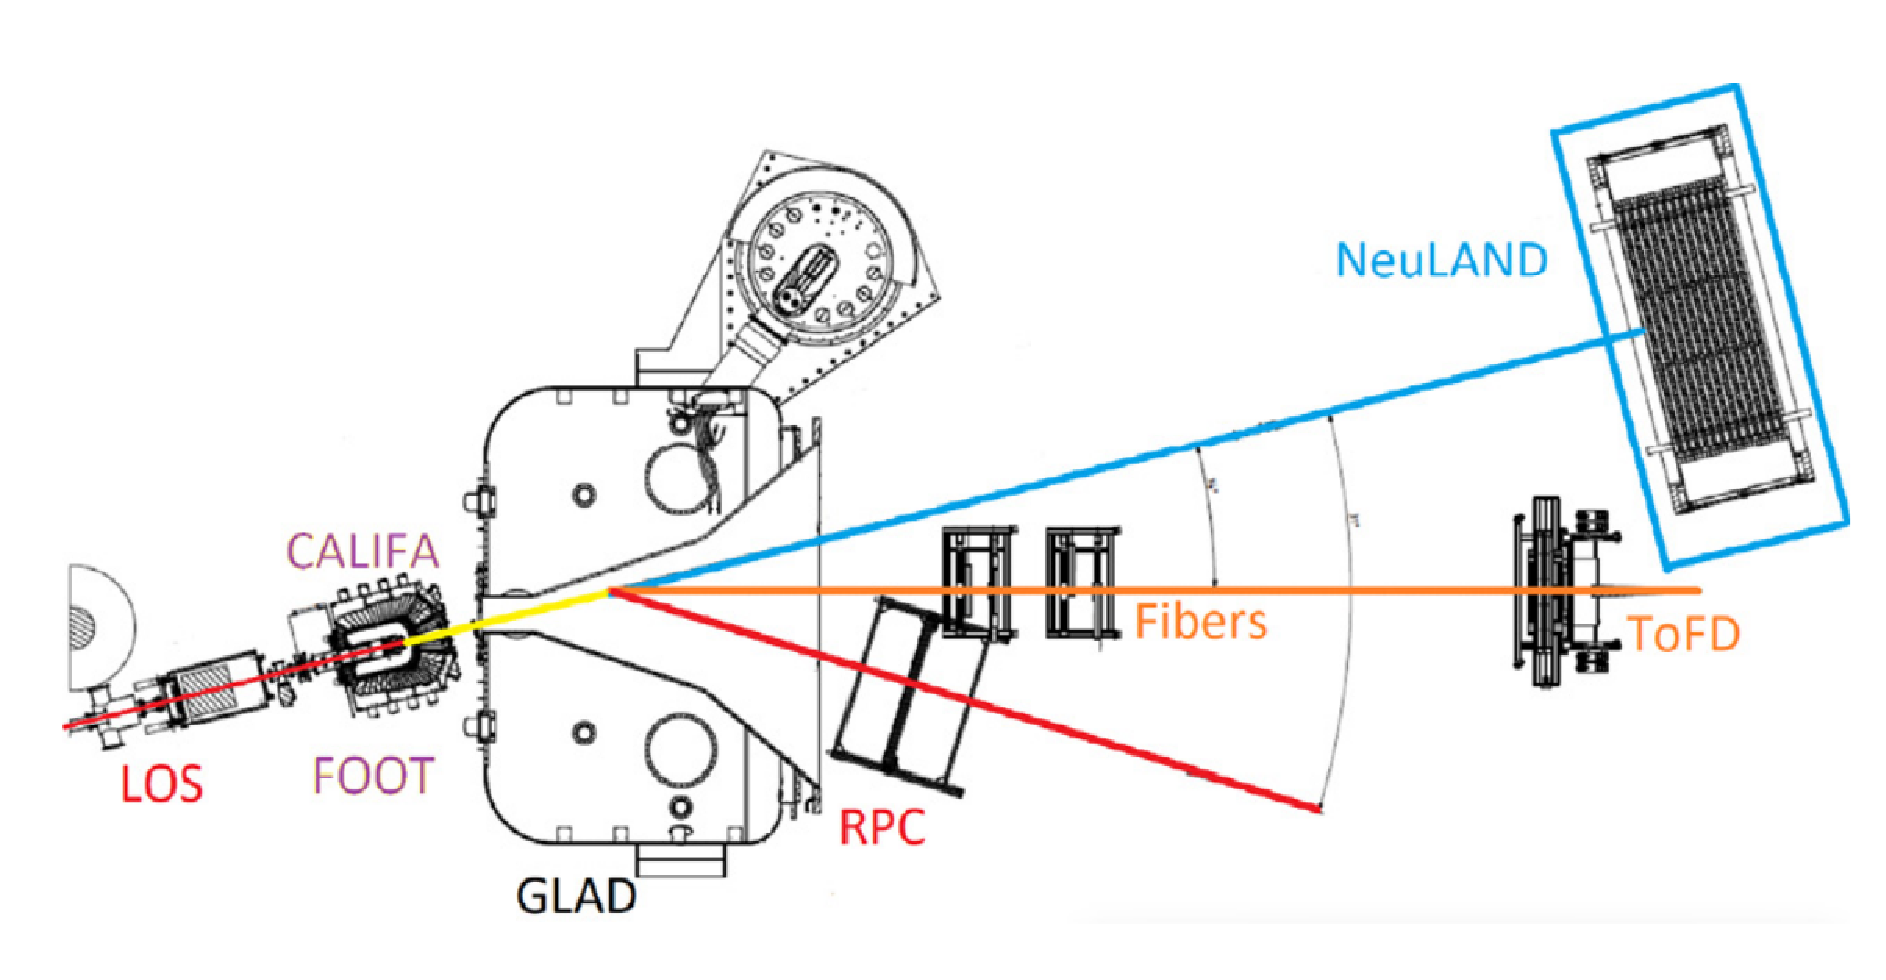
\includegraphics[width=\linewidth]{SchematicR3BSetup}
%	\caption{Schematic representation of the R$^3$B setup with beam lines.}
%	\label{fig:R3BSetup}
%\end{figure}



\subsection{Role of each detector}

\subsubsection{Beam Tracking and Initial Identification}

The experiment begins with a multi-wire proportional chamber (\textbf{MWPC}) placed at the entrance of Cave C. This detector provides coarse spatial information on the incoming secondary beam with minimal material interaction, supporting initial trajectory determination \cite{paschalis_-beam_2015}.

The \textbf{LOS}, positioned directly downstream of the MWPC, serves as the start detector for time-of-flight measurements and provides fast timing and energy-loss signals for particle identification. With a thickness of 3 mm, LOS offers good timing resolution while preserving beam quality \cite{panin2024neutron}.

Immediately following LOS, a pair of \textbf{FOOTs}—silicon-strip detectors—measure the position and energy loss of incoming ions. These detectors enable fine angular resolution and contribute to charge (Z) identification, enhancing particle-by-particle beam tagging.


\subsubsection{ALPIDE: High-Precision Pixel Tracking}

Downstream of the first FOOT pair, the beam encounters the \textbf{ALPIDE} detector. Originally developed for the ALICE ITS upgrade at CERN, ALPIDE is a monolithic active pixel sensor (MAPS) built using the 180 nm CMOS imaging process. Its architecture allows for in-pixel amplification and digitization with very low power consumption (<40 mW/cm$^2$), high spatial resolution ($\sim$ 5 $\mu$m), and detection efficiencies exceeding 99\% \cite{mager_alpide_2016}.

ALPIDE's design includes a fast, continuously active front-end and in-matrix sparsification, which minimizes data volume by transmitting only hit pixel addresses. This makes it ideal for high-rate tracking applications like \gls{R3B}. Its placement directly before the target provides excellent vertex resolution when combined with upstream and downstream tracking data.

\subsubsection{ROLU and Second FOOT Pair}

The \textbf{ROLU} acts as a beam collimation device, though not in the form of a physical absorber. Instead, it consists of four plastic scintillators arranged to define a square aperture, with the individual scintillators movable to adjust the effective beam window. The system is integrated into the trigger logic: if a particle traverses one of the scintillators, a reject signal is issued and the corresponding event is discarded. Only particles passing cleanly through the defined square aperture—without activating the scintillators—are accepted as valid events. In this way, ROLU effectively performs the role of a beam collimator by suppressing halo particles and defining the accepted beam profile, while relying purely on veto logic rather than material absorption.

Immediately after ROLU is a second pair of FOOT detectors, which reinforces the pre-target tracking and ensures consistent charge and trajectory measurements across multiple stages.

\subsubsection{Target and CALIFA}

The nuclear reaction occurs in a 50 mm liquid hydrogen (LH$_2$) target, housed in a vacuum chamber and centrally located within the \textbf{CALIFA} (CALorimeter for In-Flight particles and $\gamma$-rays) detector. CALIFA is composed of CsI(Tl) crystals in a barrel geometry surrounding the target and is designed to detect both recoil protons and γ-rays emitted from excited nuclei. Its energy resolution ($\sim$5–6\% at 1 MeV) and high granularity make it suitable for reconstructing angular distributions and reaction dynamics \cite{cortina-gil_califa_2014}.

\subsubsection{Post-Target Fragment Tracking}

Two additional FOOT pairs are placed downstream of the target: one immediately following the exit window and the other just beyond CALIFA. These silicon-strip detectors provide post-reaction trajectory and Z information for the heavy charged fragments, supporting full momentum reconstruction and enabling vertex association when correlated with upstream tracks.


\subsubsection{Magnetic Spectrometer: GLAD}

The deflection of charged fragments is performed by \textbf{GLAD} (GSI Large Acceptance Dipole), a superconducting dipole magnet optimized for large-aperture, high-rigidity measurements. Operated at reduced current for this experiment, GLAD enables separation of oxygen isotopes by their magnetic rigidity, facilitating identification of the reaction residues such as $^{22}O$, $^{23}O$ and $^{24}O$.

\subsubsection{Downstream Branches}

After GLAD, the detection branches diverge to accommodate different particle species:

\begin{itemize}
	\item Neutron Arm: Neutrons produced in the decay of unbound states travel undeviated to \textbf{NeuLAND}, a high-efficiency detector composed of 3000 plastic scintillator bars. NeuLAND offers sub-150 ps time resolution and spatial precision of $\sim$1.5 cm, allowing for accurate time-of-flight measurements and invariant-mass reconstruction in multi-neutron events. It plays a central role in identifying final states like $^{23}O + n$ and $^{22}O + 2n$.
	\item Fragment Arm: Charged fragments deflected by GLAD are tracked by four \textbf{scintillating fiber detectors}, designated Fiber 30, 31, 32 and 33. These detectors provide fine spatial resolution along the beam axis. Final time-of-flight and charge identification are performed by the \textbf{ToFD}, a four-plane plastic scintillator wall with timing precision better than 20 ps and Z resolution sufficient for fragment identification \cite{heil_new_2022}.
	\item Third Arm: A \textbf{Resistive Plate Chamber (RPC)} is also located in a separate branch downstream of GLAD. While its role in this experiment is limited to specific measurements, the RPC provides complementary timing and tracking information. A more detailed discussion of the RPC system will follow in the next chapter.
\end{itemize}


\subsection{Main DAQ}

The R3B experimental setup is integrated through a centralized \gls{DAQ} system designed to operate in a trigger-coincidence mode across all detectors. Each detector is independently connected to the main \gls{DAQ} and continuously monitors for signals corresponding to particle interactions. Upon detecting such a signal, a detector issues a trigger request to the central \gls{DAQ}. When multiple detectors generate simultaneous or time-correlated trigger requests—indicative of a valid physical event—the system recognizes this as a global trigger. In response, the \gls{DAQ} issues a trigger accept signal, prompting all participating detectors to read out and store the corresponding event data.

The digitized data from each detector are then merged into a single event stream and recorded in a common LMD (List Mode Data) file format. This format preserves the temporal correlation by organizing the information from all subsystems into event-by-event structures. To ensure consistency and temporal alignment across the detector systems, a synchronization signal is distributed at a frequency of approximately 10 Hz. This reference signal provides regular timing markers, allowing for verification and correction of potential timing drifts or misalignments during offline analysis.


\section{Personal Contribution to the Experiment}